%pdflatex -shell-escape *.tex
\documentclass{standalone}
\usepackage{amsmath,amsfonts,amssymb}
%
\usepackage{graphicx}
\graphicspath{ {images/} }
%
\usepackage{xcolor}
\pagestyle{empty}
\pagecolor{white}
%
\everymath{\displaystyle}
%
\usepackage{CJKutf8}   %CJKspace
\AtBeginDvi{\input{zhwinfonts}}
%%%
\newcommand{\zh}[1]{\begin{CJK*}{UTF8}{zhsong}#1\end{CJK*}}
\newcommand{\YBao}{\color{red}\zh{源宝爱数学}}
\newcommand{\BT}[1]{\color{red}\zh{#1}\color{black}}
\newcommand{\fTxT}[1]{\text{\zh{#1}}}
%

\immediate\write18{pdflatex complex.tex}
\immediate\write18{convert -density 150 -adaptive-resize 480x480 complex.pdf complex.jpg}
%%%
\usepackage{tikz,pgfplots}
% \pgfplotsset{height=100pt,compat=1.9}
%\usetikzlibrary{circuits.logic.US,circuits.logic.IEC}
%\usepackage{multirow}
%%%
%\usepackage{makecell}
\usepackage{tabularx}
%%%
\begin{document}\begin{minipage}[b][14cm][t]{\textwidth}
\begin{center}\Large\BT{复数}\end{center}
% \begin{tabular}{c|l}
\begin{tabularx}{\textwidth}{lX}
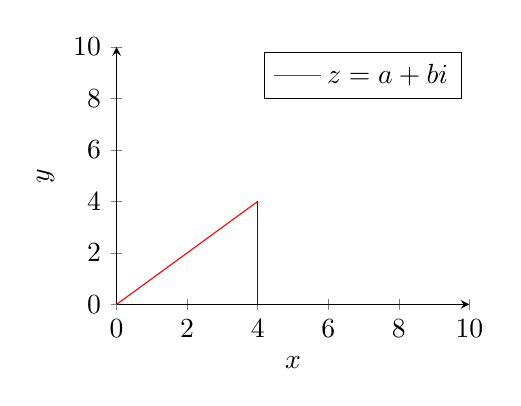
\begin{tikzpicture}[baseline=100]\begin{axis}[
  width=0.5\textwidth,height=0.4\textwidth,
  axis x line=bottom,xmin=0, xmax=10,
  xlabel={$x$},xlabel near ticks,%xticklabel style={/pgf/number format/1000 sep=},
  axis y line=left,ymin=0, ymax=10,
  ylabel={$y$}, ylabel near ticks,
  %axis on top=true,
  %axis lines=center,
  %xtick={-5,-4,...,5}, ytick={-5,-4,...,5},   
  %xlabel style={below right}, ylabel style={above left},  
  ]
  %\addplot[orange,domain=-\num:\num]{sin(deg(x))}
  \addplot [red,domain=0:4] {x};\addlegendentry{$z=a+bi$}
  \addplot [smooth,color=blue] plot coordinates {
        (4,0)
        (4,4)
    };
  \end{axis}\end{tikzpicture} &
\begin{large}\zh{i:虚数单位\color{red}$(i^2=-1)$\color{black}} \newline \zh{a:实部,b:虚部,$(a,b \in R)$} \newline \zh{模: $|z|=\sqrt{a^2+b^2}$} \newline \zh{共轭复数:$\overline{z}=a-bi$} \newline $a+bi=c+di \Leftrightarrow a=c,b=d$\end{large}

%\begin{large}\makecell{\zh{i:虚数单位\color{red}$(i^2=-1)$\color{black}} \\ \zh{a:实部,b:虚部,$(a,b \in R)$} \\ \zh{模: $|z|=\sqrt{a^2+b^2}$} \\ \zh{共轭复数:$\overline{z}=a-bi$} \\ $a+bi=c+di \Leftrightarrow a=c,b=d$}\end{large}
\\ \hline
\end{tabularx}
%\end{tabular}\\
%%%
\begin{Large}
  \begin{center}\color{blue}\zh{运算法则}\color{black}\end{center}
  \zh{四则运算} \\
  1.$(a+bi)+(c+di)=(a+c)+(b+d)i$ \\
  2.$(a+bi)-(c+di)=(a-c)+(b-d)i$ \\
  3.$(a+bi)(c+di)=(ac-bd)+(bc+ad)i$ \\
  4.$\frac{a+bi}{c+di}=\frac{ac+bd}{c^2+d^2} + \frac{bc-ad}{c^2+d^2} \hspace{3pt} (c+di \ne 0)$ \\[10pt]
  \zh{乘方运算} \\
  $z^m \cdot z^n=z^{m+n},(z^m)^n=z^{mn},(z_1 \cdot z_2)^n=z_1^n \cdot z_2^n$
\end{Large}
%%%
\end{minipage}\end{document}
%%% 
